\documentclass[10pt,hyperref={CJKbookmarks=true},xcolor=dvipsnames,aspectratio=169]{beamer}
\usetheme[navigation]{UMONS}
\usepackage[utf8]{inputenc}
\usepackage{verbatim}
\usepackage{ctex}

\title[国际经济学]{国际经济学}
\subtitle{规模经济与国际贸易:新贸易理论}
\author{鲁晓东}
\institute[]{%
	岭南学院\hspace{2em}中山大学
	\\[4ex]
	
\includegraphics[height=8ex]{fig/lingnanlogo}\hspace{2em}%
	
\includegraphics[height=8.5ex]{fig/sysu}
}
%------------section前展示一页----------
\AtBeginSection[] {     
	\begin{frame}        
	\tableofcontents[currentsection,hideallsubsections]    
\end{frame} 
}

%-------------subsection也展示一下----------
\AtBeginSubsection[]{

\frame<beamer>{ 
	
	\frametitle{Outline}   
	
	\tableofcontents[currentsection,currentsubsection] 
	
}

}
%---------------------------

%-----------一段一闪现-------
%\beamerdefaultoverlayspecification{<+->}
%这个功能基本不用

\begin{document}
\maketitle


\begin{frame}
\frametitle{提纲}
\tableofcontents
\end{frame}				%生成提纲页

%-----------正文开始----------------------



\section{Motivation}
\begin{frame}{Motivation: a Surprising Kind of Trade}

\begin{itemize}
\item We will look at trade in \textbf{\textcolor{red}{golf clubs}}, a good
that the U.S. \textbf{\textcolor{red}{imports and exports in large
quantities}}.
\item Many countries that sell to the U.S. are also buying from the U.S. 

\begin{itemize}
\item The total value of imports is close to the total value of exports.
\end{itemize}
\item Why does the U.S. export and import golf clubs to and from the same
countries? 

\begin{itemize}
\item We observe \textbf{\textcolor{red}{intra-industry trade}}. 产业内贸易
\item A new explanation for trade will be discussed here. 
\end{itemize}
\end{itemize}
\end{frame}

\begin{frame}{The data:}


\begin{figure}
\protect\caption{U.S. Imports and Export of Golf Clubs, 2005}


\centering{}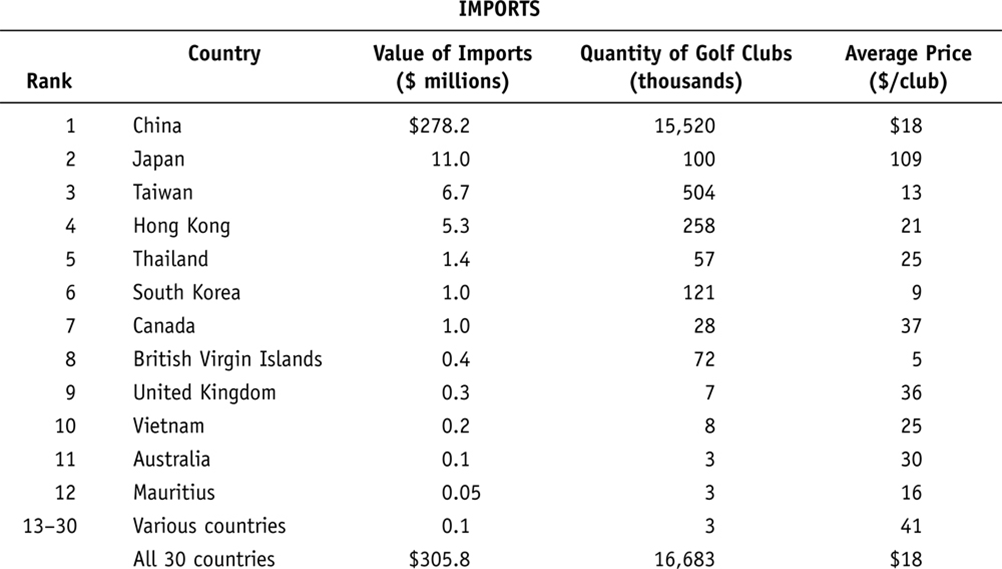
\includegraphics[width=7.5cm]{fig/krugman/lec6-1}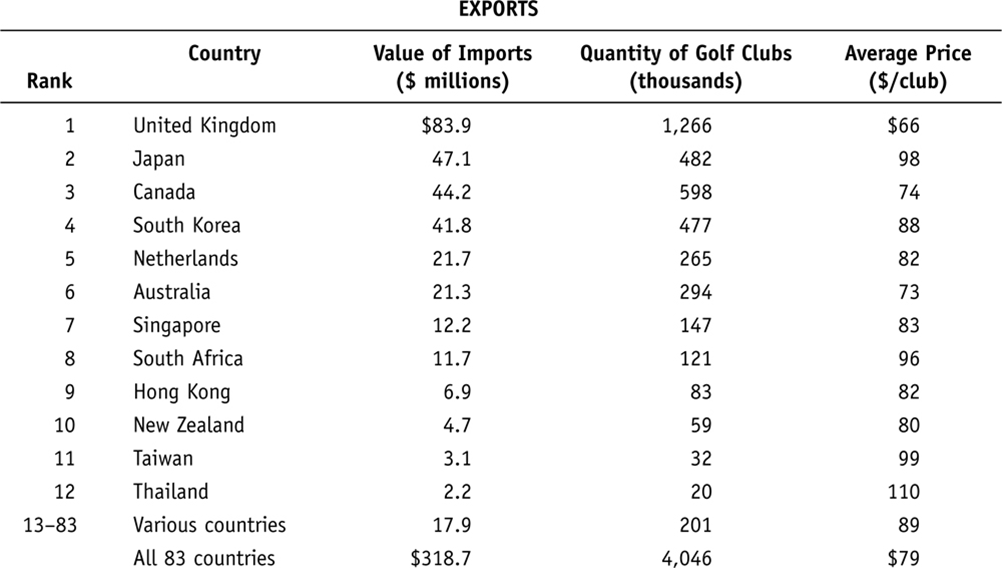
\includegraphics[width=7.5cm]{fig/krugman/lec6-2}
\end{figure}

\begin{itemize}
\item Very hard to explain this with models we have used so far 
\item As we will later see, \textbf{\textcolor{red}{increasing returns to
scale}} are fundamental force behind this phenomenon
\end{itemize}
\end{frame}

\begin{frame}{Broader Motivation}

\begin{itemize}
\item The models we have developed so far emphasize \textbf{\textcolor{red}{cross
-country differences}} in autarky prices as sources of trade 
\item These autarky price differences may stem from technology differences
(Ricardian model) or from factor endowment differences (Heckscher-Ohlin
model) 
\item Regardless, countries trade because they are different 
\item However, \textbf{\textcolor{red}{the majority of world trade is between
similar countries}} 

\begin{itemize}
\item Similar technologies, similar endowments 
\end{itemize}
\item How do we explain this? 
\end{itemize}
\end{frame}

\begin{frame}{Interindustry vs. Intraindustry Trade }

\begin{itemize}
\item Similarly, the models so far emphasize an intersectoral nature of
trade flows (cloth for food) 
\item In reality, a large fraction of world trade is intraindustry trade
\item Measuring intra-industry trade: the Grubel-Lloyd (GL) index 
\[
IIT_{i}=GL_{i}=1-\frac{|Ex_{i}-Im_{i}|}{Ex_{i}+Im_{i}}
\]
\begin{figure}
\centering{}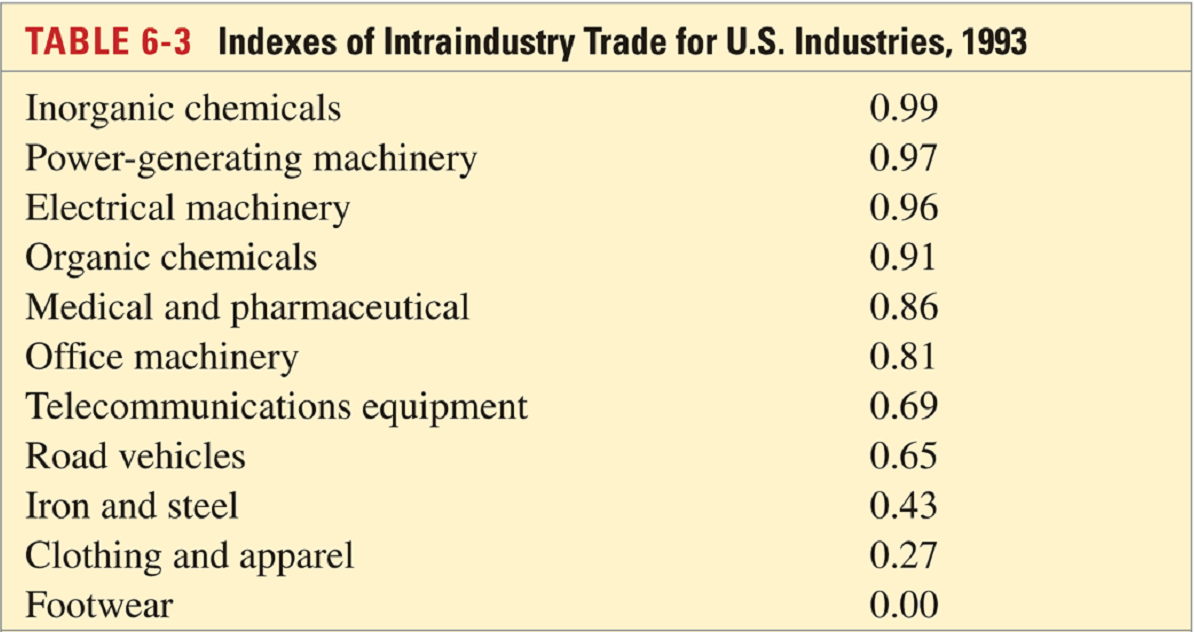
\includegraphics[width=8cm]{fig/krugman/lec6-3}
\end{figure}

\end{itemize}
\end{frame}

\begin{frame}{“New” Trade Theory 新贸易理论 }

\begin{itemize}
\item Trade theory since the late 1970s has pushed the view that \textbf{\textcolor{red}{imperfect
competition and increasing returns to scale}} 不完全竞争和规模报酬递增 may be
key in explaining the actual features of trade flows 

\begin{itemize}
\item Krugman received the 2008 Nobel Prize for these developments
\end{itemize}
\item Broadly speaking, imperfect competition will imply that \textbf{\textcolor{red}{two-
way trade flows}} within the same industry will become possible 
\item Increasing returns to scale will imply that \textbf{\textcolor{red}{country
size}} will become a determinant of comparative advantage 如何理解此处的比较优势?
\item 这是否让你想起了之前讨论的Orphan——引力方程,它们之间有什么关联吗?
\end{itemize}
\end{frame}

\begin{frame}{Increasing Returns to Scale }

\begin{itemize}
\item Previous models assumed \textbf{\textcolor{red}{constant returns to
scale}}: 

\begin{itemize}
\item If all factors of production are doubled then output will also double 
\end{itemize}
\item But a firm or industry may feature \textbf{\textcolor{red}{increasing
returns to scale}} (or economies of scale ) 
\item A production technology exhibits IRS if an $x$\% increase in all
factors leads to more than $x$\% increase in output 

\begin{itemize}
\item This implies that Average Cost (AC) decreases as output increases 
\item Production is more efficient if it takes place on a larger scale 
\end{itemize}
\item Economies of Scale comes in two varieties 规模经济的两种类型

\begin{itemize}
\item \textbf{\textcolor{red}{Internal:}} AC of firm falls with firm output
内部规模经济
\item \textbf{\textcolor{red}{External:}} AC of firm falls with industry
output 外部规模经济
\end{itemize}
\end{itemize}
\end{frame}

\begin{frame}{An Example}


\begin{columns}[onlytextwidth]
\begin{column}{0.5\textwidth}
\begin{itemize}
\item Assume labor is the only input required 
\item Note that the average amount of inputs needed to produce output declines
as the volume of output (at the firm or industry level) increases 
\item \textbf{\textcolor{red}{Example}}: internal IRS may arise because
there is an overhead cost of 5 units of labor (regardless of output) 
\end{itemize}

\end{column}
\begin{column}{0.5\textwidth}
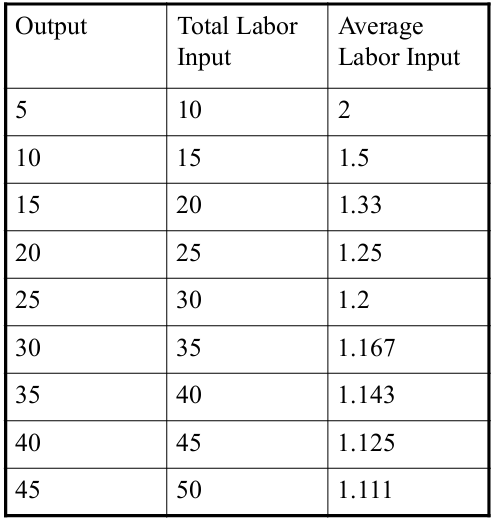
\includegraphics[width=0.9\columnwidth]{fig/krugman/lec6-4}
\end{column}
\end{columns}

\end{frame}

\begin{frame}{Benefits from Trade: Preview }

\begin{itemize}
\item Imagine that there are two goods A and B with the production technique
described above 
\item If a country assigns 15 workers to each good, then they get 10 units
of each good (so world produces 20 units of each good) 
\item Instead, suppose a country assigns its 30 workers to the production
of only one good 怎样多找15个人来生产这种产品?
\item Then production is 25 units of that good 
\end{itemize}

\pause{}
\begin{itemize}
\item Suppose another country does the same and specializes in the other
good 
\item World is now producing 25 units of each variety (before 20)
\end{itemize}
\end{frame}

\begin{frame}{Possible Losses from Trade: Preview}

\begin{itemize}
\item Imagine that there is an IRS good A with technology described above,
and a second good B produced one-to-one from labor 
\item Suppose one country (Home) has 50 workers and the other country (Foreign)
has 20 workers 
\item If in autarky each country has half of its workforce in each sector: 

\begin{itemize}
\item Home produces 20 units of A and 25 units of B 
\item Foreign produces 5 units of A and 10 units of B 
\end{itemize}
\item Suppose now that Home specializes in B and Foreign in A 

\begin{itemize}
\item Then world produces 15 units of A and 50 units of B 
\end{itemize}
\item World output of good B is higher, but that of good A is lower 

\begin{itemize}
\item If consumers value good A sufficiently, world welfare is reduced 
\end{itemize}
\end{itemize}
\end{frame}

\begin{frame}{IRS and Market Structure}

\begin{itemize}
\item Modeling increasing returns to scale poses difficulties for how to
treat market structure 规模报酬递增下对应着怎样的市场结构?
\item Is it still sensible to work with perfectly competitive markets? 
\item The nature of the external economies has important implications for
the structure of industries: 

\begin{itemize}
\item An industry where economies of scale are purely external will typically
consist of many small firms and be perfectly competitive 外部规模经济可能对应完全竞争市场
\item Internal economies of scale result when large firms have a cost advantage
over small firms, causing the industry to become imperfectly competitive
内部规模经济意味着某些企业的规模大于行业平均规模,从而获得了一定的垄断力量
\end{itemize}
\item Hence, external economies of scale are a natural starting point 因此,我们从外部规模经济说起
\end{itemize}
\end{frame}



\section{External Economies of Scale }
\begin{frame}{Intellectual History}


\begin{columns}[onlytextwidth]
\begin{column}{0.4\textwidth}
\begin{itemize}
\item \textbf{\textcolor{red}{External economies of scale }}were first defined
by Alfred Marshall (1842 -1924) 
\item Their implications for trade patterns and welfare were studied by
Frank Graham (1890 - 1949) 
\end{itemize}

\end{column}
\begin{column}{0.6\textwidth}
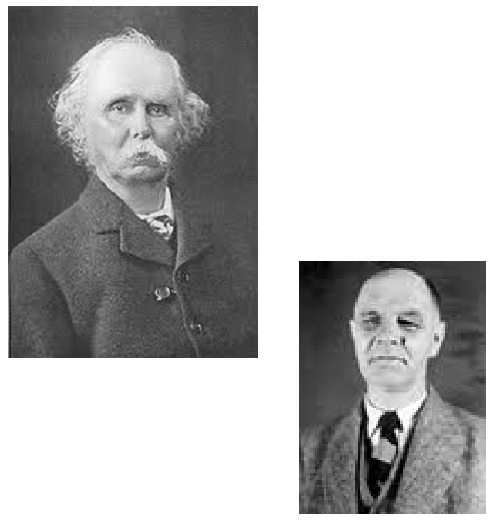
\includegraphics[width=0.8\columnwidth]{fig/krugman/lec6-5}
\end{column}
\end{columns}

\end{frame}

\begin{frame}{External Economies of Scale }

\begin{itemize}
\item Remember that external economies of scale arise when average costs
are decreasing in the output of other firms in the industry or in
the economy 
\item If external economies exist, a country or region that has a large
industry will have low costs of producing that industry’s good or
service 
\item Marshall thought that the source of external economies of scale are:

\begin{itemize}
\item Specialized Suppliers
\item Labor Market Pooling
\item Knowledge Spillovers
\end{itemize}
\end{itemize}
\end{frame}

\begin{frame}{Examples }

\begin{itemize}
\item In the US, the semiconductor industry is concentrated in Silicon Valley,
investment banking in New York, and the entertainment industry in
Hollywood 
\item In developing countries, external economies are pervasive in manufacturing 

\begin{itemize}
\item One town in China produces most of the world’s underwear, another
nearly all cigarette lighters 
\item One town in Pakistan (Sialkot) produces 70\% of world soccer balls 
\item Indian information services companies are still clustered in Bangalore 
\end{itemize}
\end{itemize}
\end{frame}

\begin{frame}{External Economies of Scale}

\begin{itemize}
\item External economies may exist for several reasons: 

\begin{enumerate}
\item Specialized equipment or services may be needed for the industry,
but are only supplied by other firms if the industry is large and
concentrated (e.g., Silicon Valley firms serviced by machine producers) 
\item Labor pooling: a large and concentrated industry may attract a pool
of workers, reducing labor search and hiring costs for all firms in
the industry 
\item Knowledge spillovers: a large and concentrated industry may facilitate
the sharing of productive ideas between workers in different firms 
\end{enumerate}
\end{itemize}
\end{frame}

\begin{frame}{Implications for Industry Equilibrium}


\begin{columns}[onlytextwidth]
\begin{column}{0.6\textwidth}
\begin{itemize}
\item There is a \textbf{\textcolor{red}{forward-falling supply curve}}:
the larger the industry’s output, the lower the price at which firms
are willing to sell 
\item Without international trade, the unusual slope of the supply curve
might not matter much 为什么外部规模经济在国际贸易的情况下更容易发生?
\end{itemize}

\end{column}
\begin{column}{0.4\textwidth}
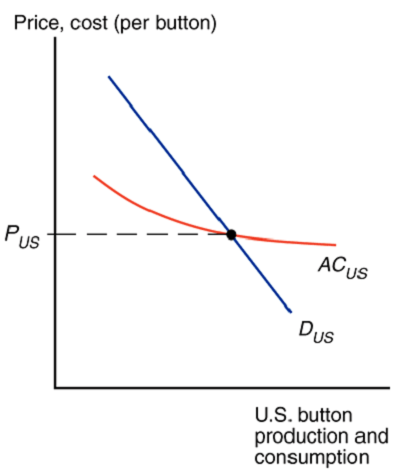
\includegraphics[width=\columnwidth]{fig/krugman/lec6-6}
\end{column}
\end{columns}

\end{frame}

\begin{frame}{Differences in Autarky Prices }

\begin{itemize}
\item As an example, consider the button industry
\begin{figure}
\centering{}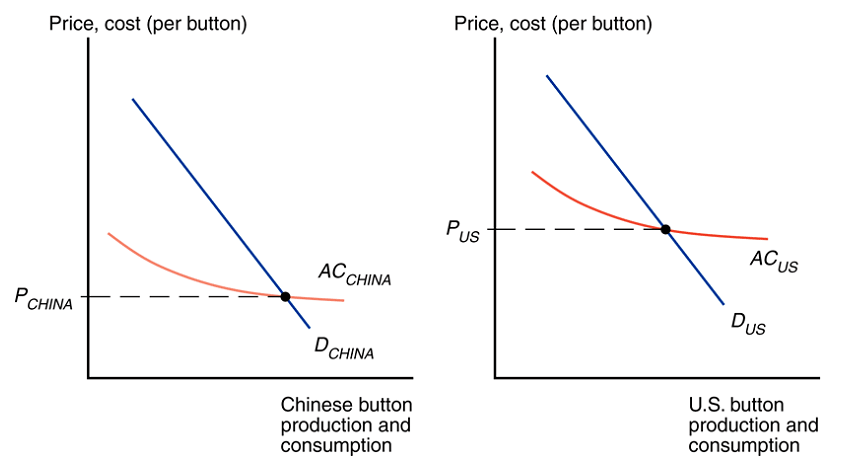
\includegraphics[width=10cm]{fig/krugman/lec6-7}
\end{figure}

\end{itemize}
\end{frame}

\begin{frame}{External Scale Economies and Trade}

\begin{itemize}
\item What will happen when the countries open up the potential for trade
in buttons? 
\item The Chinese button industry will expand, while the U.S. button industry
will contract 
\item As the Chinese industry’s output rises, its costs will fall further;
as the U.S. industry’s output falls, its costs will rise 
\item In the end, all button production will be in China 
\end{itemize}
\end{frame}

\begin{frame}{Trade and Prices}


\begin{columns}[onlytextwidth]
\begin{column}{0.5\textwidth}
\begin{itemize}
\item Because supply curve is forward-falling, increased production as a
result of trade leads to a button price that is lower than the price
before trade 
\item Trade leads to prices that are\textbf{\textcolor{red}{{} lower}} than
the prices\textbf{\textcolor{red}{{} in either country}} before trade!
\end{itemize}

\end{column}
\begin{column}{0.5\textwidth}
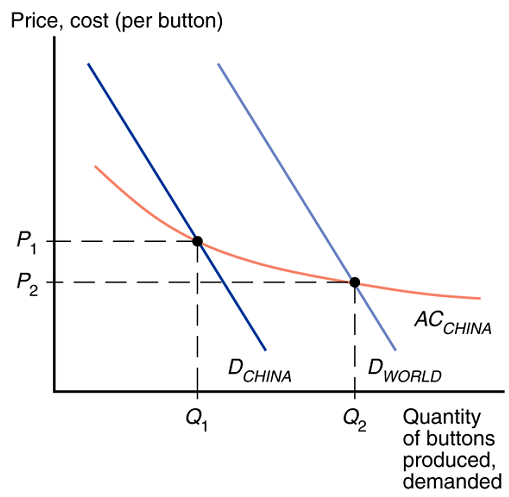
\includegraphics[width=\columnwidth]{fig/krugman/lec6-8}
\end{column}
\end{columns}

\end{frame}

\begin{frame}{Trade and Prices (cont.) }

\begin{itemize}
\item Note the very different implications relative to models without increasing
returns. 与以前贸易模型的显著差异是:价格的变化趋势
\item In the standard trade model relative prices converge as a result of
trade 

\begin{itemize}
\item They go up for goods that were abundant under autarky and down for
goods that were scarce 在自给自足情况下生产规模大的产品的相对价格会上升,反则反之 
\end{itemize}
\item With external economies, by contrast, the effect of trade is to reduce
prices\textbf{\textcolor{red}{{} everywhere 而在外部经济的情况下,都会下降!}}
\end{itemize}
\end{frame}

\begin{frame}{Determinants of Comparative Advantage}


\begin{columns}[onlytextwidth]
\begin{column}{0.5\textwidth}
\begin{itemize}
\item If external economies exist, the pattern of trade may be due to \textbf{\textcolor{red}{historical
accidents}} 贸易模式由历史的偶然因素决定的
\item In the graph, Vietnam could manufacture buttons more cheaply than
China at any given level of production 
\item But with zero production in Vietnam, the average cost is higher than
the initial price, which is $P_{1}$
\end{itemize}

\end{column}
\begin{column}{0.5\textwidth}
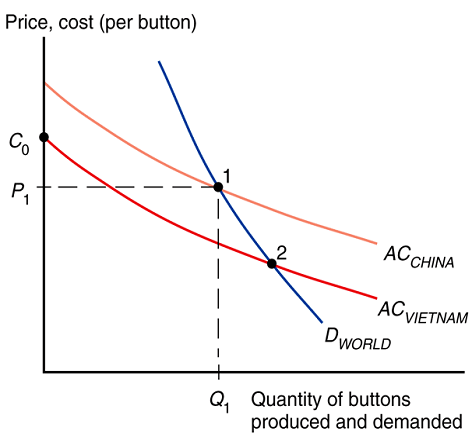
\includegraphics[width=\columnwidth]{fig/krugman/lec6-9}
\end{column}
\end{columns}

\end{frame}

\begin{frame}{Welfare Effects of Trade}

\begin{itemize}
\item Trade based on external economies has an \textbf{\textcolor{red}{ambiguous
effect }}on national welfare 对国家福利的影响是含混的
\item There may be gains to the world economy of concentrating production
of industries with external economies 
\item But where does production concentrate? It may seem optimal to concentrate
it in the most efficient countries 生产区位理论
\item But as the example above illustrated, there is no guarantee this will
happen 
\item As a result, in some cases some countries might be worse off with
international trade than without it (Graham, 1928) 某些国家会因国际贸易而受损,为什么?
\end{itemize}
\end{frame}

\begin{frame}{A Graphical Example }


\begin{columns}[onlytextwidth]
\begin{column}{0.5\textwidth}
\begin{itemize}
\item Suppose Thailand can produce watches more cheaply than Switzerland,
but only the latter produces them (for historical reasons) 
\item Thailand cannot profitably enter 
\item But if Thailand restricts trade in watches… 限制性贸易政策有了存在的意义
\item … they will end up consuming them at a lower price $P_{2}<P_{1}$ 
\end{itemize}

\end{column}
\begin{column}{0.5\textwidth}
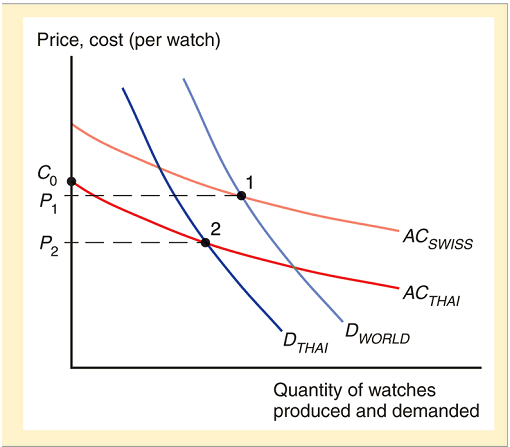
\includegraphics[width=\columnwidth]{fig/krugman/lec6-10}
\end{column}
\end{columns}

\end{frame}

\begin{frame}{Dynamic External Economies of Scale}

\begin{itemize}
\item We have considered cases where external economies depend on the amount
of \textbf{\textcolor{red}{current output }}at a point in time 关键看你现在是否已经生产,已经生产的规模
\item \textbf{\textcolor{red}{Dynamic external economies of scale}} (dynamic
IRS) exist if average costs fall as \textbf{\textcolor{red}{cumulative
output}} increases over time 动态收益递增
\item Think about a process of accumulation of knowledge or experience 知识和经验的积累
\item A graphical representation of dynamic increasing returns to scale
is called a \textbf{\textcolor{red}{learning curve 学习曲线以及干中学理论 }}
\item Especially important in some high-tech industries, such as aeronautics
\end{itemize}
\end{frame}

\begin{frame}{Dynamic External Economies of Scale }


\begin{columns}[onlytextwidth]
\begin{column}{0.5\textwidth}
\begin{itemize}
\item Dynamic external IRS have the same implications as static external
IRS 

\begin{itemize}
\item History may matter 
\item Protectionism may be justified 
\end{itemize}
\item The latter is related to the so - called \textbf{\textcolor{red}{“infant-industry}}”
argument for protection 幼稚工业理论的缘起和发展
\item \textbf{\textcolor{red}{Key issue}}: which industries should be protected
and for how long? 幼稚工业理论的阿克琉斯之踵
\item 对我们的启示:有些事情可以先做起来
\end{itemize}

\end{column}
\begin{column}{0.5\textwidth}
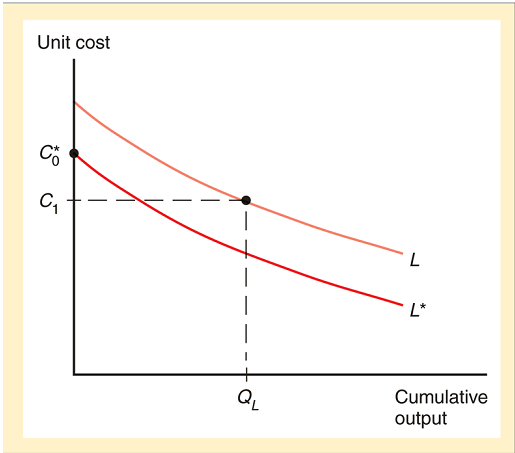
\includegraphics[width=\columnwidth]{fig/krugman/lec6-11}
\end{column}
\end{columns}

\end{frame}

\begin{frame}{Implications for Policy: Preview }

\begin{itemize}
\item Governments may want to actively encourage investment in technology
when externalities in new technologies create a high marginal social
benefit 
\item When considering whether a government should subsidize high-technology
industries, should consider: 

\begin{enumerate}
\item The ability of government to subsidize the right activity 
\item Instead of subsidizing specific industries, it may be better to subsidize
research and development through the tax code 
\item The economic importance of externalities (measurable?) 
\item Externalities may occur across countries as well (free-riding) 
\end{enumerate}
\end{itemize}
\end{frame}



\section{Internal Economies of Scale }
\begin{frame}{Internal Economies of Scale }

\begin{itemize}
\item When economies of scale are internal, large firms may be more efficient
than small firms, and the industry may consist of a monopoly or a
few large firms 市场结构发生变化
\item This creates a tension with the notion of perfect competition: 

\begin{itemize}
\item many buyers and sellers, all price takers 
\item sellers can sell/supply as much as they want at the current price
without worrying about driving the price down 
\end{itemize}
\item Not a good assumption when only a few firms produce a good 

\begin{itemize}
\item Ex: in the aircraft industry, both Boeing and Airbus know that if
they produce more, they will have a significant effect on total aircraft
supply, thus driving the price down 
\end{itemize}
\end{itemize}
\end{frame}

\begin{frame}{Imperfect Competition }

\begin{itemize}
\item More natural to assume that the industry is \textbf{\textcolor{red}{imperfectly
competitive}}
\item In imperfectly competitive markets, the quantity they produce will
influence the price it sells for, i.e. $P(Q_{i})$ with $P\prime(Q_{i})<0$ 
\item How the price is influenced generally depends on industry demand and
market structure 
\item Note also that, under perfect competition, firms would operate at
the point in which Price = Marginal Cost, but then with IRS the firm
would not be able to cover the higher costs incurred from producing
the initial units of output 难以越过刚刚开始生产时的高成本,为什么?成本函数怎么写?
\end{itemize}
\end{frame}

\begin{frame}{The Monopolist Problem}

\begin{itemize}
\item In such a case, $P(Q)$ is simply the inverse of the market demand
curve (determined by consumer preferences, not the industrial structure
与产业结构无关) 
\item Demand is downward-sloping, with an elasticity that depends on the
degree to which the monopolist’s output is substitutable with other
different products 需求曲线的倾斜程度
\item Marginal revenue slopes down also, and always lies below the demand
curve 为什么?
\item Total Revenue = $P(Q)\cdot Q$
\item Marginal Revenue = $P(Q)+P\prime(Q)\cdot Q<P(Q)$ 
\end{itemize}
\end{frame}

\begin{frame}{Cost Structure }

\begin{itemize}
\item Suppose that the total costs of the monopolist are $TC=F+cQ$, 
\item $F$ represents a fixed or overhead cost (and is independent of the
level of output) 
\item $c$ represents a constant marginal cost: the constant cost of producing
an additional unit of output $Q$ 
\item Average cost is then: $AC=F/Q+c$ 
\item A larger firm is more efficient because average cost decreases as
output $Q$ increases:\textbf{\textcolor{red}{{} internal economies
of scale}}
\end{itemize}
\end{frame}

\begin{frame}{Optimal Scale of Operation}

\begin{itemize}
\item The monopolist will choose the scale of operation that maximizes profits 
\item Namely a $Q$ s.t. that $[P(Q)\cdot Q-F-cQ]$
is maximized 
\item This implies $MR(Q^{*})=MC(Q^{*})=c$ 
\item Note that the optimal price satisfies $P^{*}=P(Q^{*})>c$ 
\item And optimal profits equal $P(Q^{*})\cdot Q^{*}-F-cQ^{*}$
\end{itemize}
\end{frame}

\begin{frame}{Graphical Analysis}


\begin{columns}[onlytextwidth]
\begin{column}{0.5\textwidth}
\begin{itemize}
\item Suppose the demand curve the firm faces is a straight line $Q=A-BP$,
where $A$ and $B$ are constants. 
\item \textbf{\textcolor{red}{Marginal revenue}} equals $MR=P-Q/B$
. 
\end{itemize}

\end{column}
\begin{column}{0.5\textwidth}
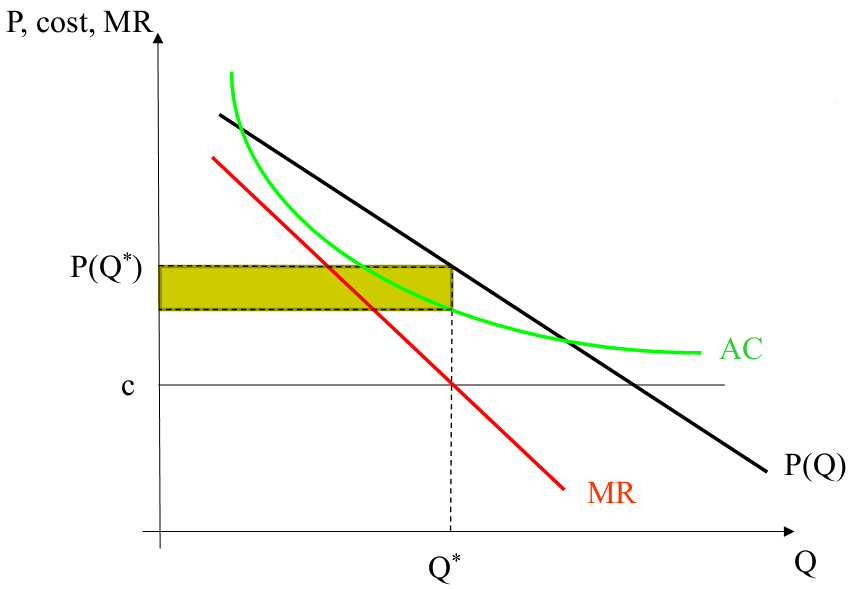
\includegraphics[width=\columnwidth]{fig/krugman/lec6-12}
\end{column}
\end{columns}


\end{frame}

\begin{frame}{Oligopolistic Competition }

\begin{itemize}
\item One rarely sees only one producer per good (e.g. a natural resource
that only one firm has access to) 完全垄断
\item If there are a small number of very large producers (\textbf{\textcolor{red}{oligopoly}}),
we can use game -theoretic tools to model their interactions, as their
pricing decisions are interdependent 
\item But this can get very complicated, as we have to take into account
how firms second-guess the behavior of their competitors 寡头分析从技术上讲比较困难
\item Alternatively, we can model multi-firm imperfect competition via “\textbf{\textcolor{red}{monopolistic
competition}}”, which gets around the interdependence issue 只分析垄断竞争的情况
\end{itemize}
\end{frame}



\section{Monopolistic Competition}
\begin{frame}{Intellectual History }


\begin{columns}[onlytextwidth]
\begin{column}{0.5\textwidth}
\begin{itemize}
\item Developed by Paul Krugman (1953- ) using a model of industry equilibrium
first suggested by Edward Chamberlin (1899 - 1967)
\end{itemize}

\end{column}
\begin{column}{0.5\textwidth}
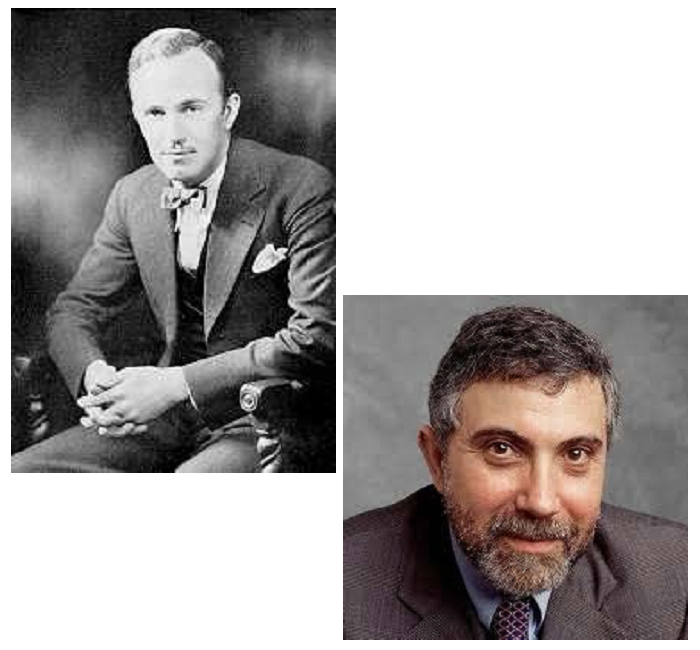
\includegraphics[width=\columnwidth]{fig/krugman/lec6-13}
\end{column}
\end{columns}


\end{frame}

\begin{frame}{Monopolistic Competition }

\begin{itemize}
\item Due to Chamberlin (1933), its distinctive features are: 

\begin{enumerate}
\item Each firm has some market power in the sense that it faces a downward-
sloping demand curve 每个厂商都有一定的垄断力
\item There are a large number of firms so that a price change by a single
firm has no effect on the level of demand faced by the rest of the
firms 行业内有大量企业
\item There is free entry so that firm profits are driven down to zero 行业自由进出,且利润为0
\end{enumerate}
\end{itemize}
\end{frame}

\begin{frame}{Free Entry at Work }


\begin{figure}
\centering{}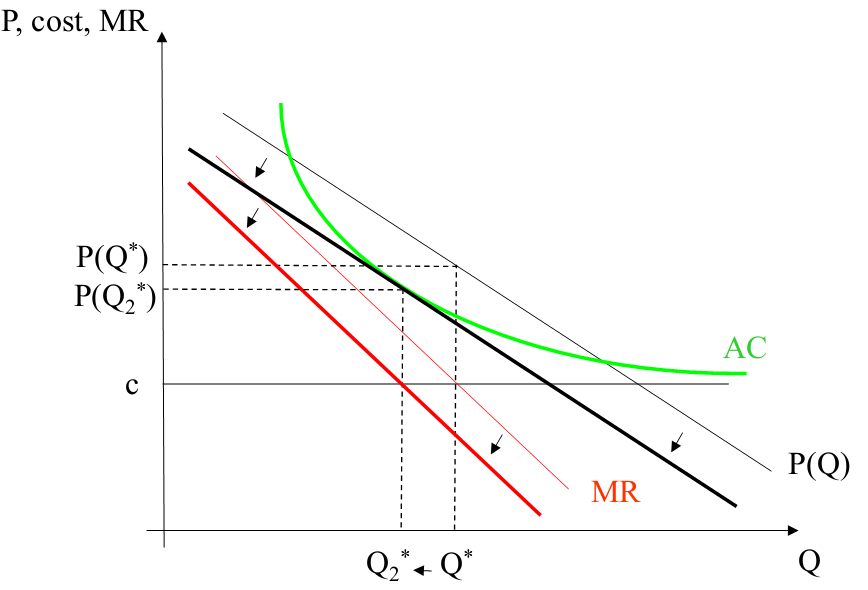
\includegraphics[width=10cm]{fig/krugman/lec6-14}
\end{figure}



\end{frame}

\begin{frame}{Product Differentiation 差异产品}

\begin{itemize}
\item Where does the downward sloping demand function come from? 
\item There can be many firms within an industry, but each firm can differentiate
its product (e.g. Samsung Galaxy vs. Apple iPhone) 
\item It is important that consumers value that the economy provides \textbf{\textcolor{red}{a
variety of differentiated products }}

\begin{itemize}
\item Perhaps consumers themselves value variety (Dixit- Stiglitz, 1977)
多样化偏好
\item Or different consumers value different varieties (Lancaster, 1979)
差异品的理想多样化,每个人都有一个“ideal variety”
\end{itemize}
\item In sum, each individual producer behaves like a monopolist but free
entry drives profits down to zero 
\end{itemize}
\end{frame}

\begin{frame}{Example}

\begin{itemize}
\item Suppose we represent the demand faced by a differentiated-good producer
by
\[
Q=S\text{·}[1/n\text{–}b(P\text{–}P_{avg})]
\]

\item $Q$ is the quantity sold by the firm 
\item $S$ are total sales (in quantity terms) of the industry 常数 
\item $n$ is the number of firms in the industry 
\item $b$ captures the responsiveness of a firm’s sales to its price 常数,表示公司的销量对价格变化的反应程度
\item $P$ is the price charged by the firm itself 
\item $P_{avg}$is the average price charged by its competitors 
\item 考虑:如果厂商都制定相同价格;如果价格高于平均水平;如果价格低于平均水平
\end{itemize}
\end{frame}

\begin{frame}{Example (cted.)}

\begin{itemize}
\item Assume that firms are \textbf{\textcolor{red}{symmetric}}(representive
firm, leave room for the heterogenous firm trade theory: all firms
face the same demand function and have the same cost function, so
in equilibrium $P=P_{avg}$ 
\item Then $Q=S/n$ , and firms get the same market share 
\item If instead, we had $P>P_{avg}$ , then the firm would still have a
positive market share, but it would be lower than $1/n$ 
\item Hence demand is downward sloping (not perfectly elastic), unless $b\rightarrow\infty$
\item 求解:行业中厂商的数量$n$和代表性价格$P_{avg}$
\end{itemize}
\end{frame}

\begin{frame}{Optimal Pricing }

\begin{itemize}
\item Remember that each firm acts like a monopolist, and hence $Q$ (or
$P$) is chosen such that $MR=MC=c$ 
\item We first invert the demand function: 
\[
P=P_{avg}+1/(nb)\text{–}Q/(Sb)
\]
 
\item Then we compute 
\[
MR=P(Q)+P^{\text{'}}(Q)\text{·}Q=P\text{–}Q/(Sb)
\]

\item Now note that in equilibrium, $Q=S/n$
\item So we have 由零利润条件推导出 
\[
P=c+1/(nb)\begin{array}{ccccc}
 &  &  &  & \left({\color{red}PP}\right)\end{array}
\]

\item 反应了产品价格和厂商数量之间的关系
\end{itemize}
\end{frame}

\begin{frame}{Average Costs }

\begin{itemize}
\item In a symmetric equilibrium, we must have 
\[
Q=S/n
\]
 
\item But then, average cost is equal to 由成本函数推出
\[
AC=TC/Q=F/Q+c=F\text{·}n/S+c\begin{array}{ccccc}
 &  &  &  & \left({\color{red}CC}\right)\end{array}
\]
 反应了生产成本和厂商数量的关系
\item The larger the number of firms n , the higher $AC$ for each firm
because each firm produces less 
\item The larger total industry sales S , the lower $AC$ for each firm
because each firm produces more 
\end{itemize}
\end{frame}

\begin{frame}{Equilibrium }


\begin{columns}[onlytextwidth]
\begin{column}{0.5\textwidth}
\begin{itemize}
\item Graphically, we can pin down $P$ and $n$ as the intersection of
( \textbf{\textcolor{red}{CC}}) and ( \textbf{\textcolor{red}{PP}}) 
\item At $n_{1}$ , $P>AC$ and there is an incentive for entry 

\begin{itemize}
\item An increase in $n$, reduces prices (competition) and increases $AC$ 
\end{itemize}
\item In some case, this model was named \textbf{\textcolor{red}{PP-ZZ model}}
\end{itemize}

\end{column}
\begin{column}{0.5\textwidth}
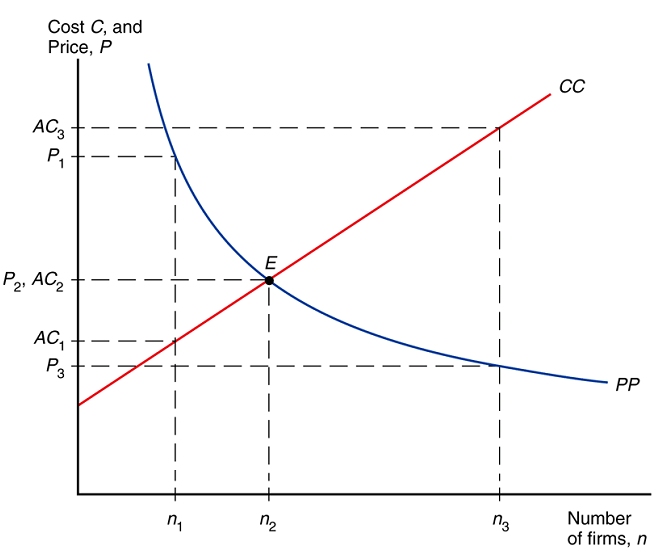
\includegraphics[width=\columnwidth]{fig/krugman/lec6-15}
\end{column}
\end{columns}


\end{frame}

\begin{frame}{Monopolistic Competition and Trade: an Application of PP-ZZ Model}

\begin{itemize}
\item Remember the key equations of the monopolistic competition model 
\end{itemize}
\[
AC=TC/Q=F/Q+c=F\text{·}n/S+c\begin{array}{ccccc}
 &  &  &  & ({\color{red}CC})\end{array}
\]


\[
P=c+1/(nb)\begin{array}{ccccc}
 &  &  &  & ({\color{red}PP})\end{array}
\]

\begin{itemize}
\item These two equations yield a solution for $P$ and $n$ 
\item What is the effect of trade? 
\item Suppose trade increases market size, so S goes up 
\item No effect on (\textbf{\textcolor{red}{PP}}) curve, while (\textbf{\textcolor{red}{CC}})
curve shifts down 

\begin{itemize}
\item No direct effect on optimal pricing, but $AC$ will tend to go down 
\end{itemize}
\end{itemize}
\end{frame}

\begin{frame}{Graphical Analysis }


\begin{columns}[onlytextwidth]
\begin{column}{0.5\textwidth}
\begin{itemize}
\item The shift in the CC curve will lead to a larger number of firms in
the industry and to lower equilibrium prices 
\item Hence, there is a pro-competitive effect and a variety - enhancing
effect 
\item Note that consumers (or society) value variety, so both effects are
welfare-enhancing
\end{itemize}

\end{column}
\begin{column}{0.5\textwidth}
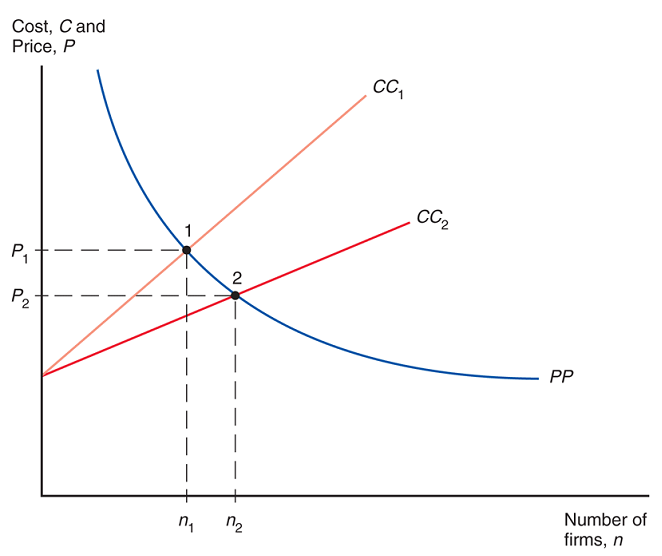
\includegraphics[width=\columnwidth]{fig/krugman/lec6-16}
\end{column}
\end{columns}




\end{frame}

\begin{frame}{Numerical Example }

\begin{itemize}
\item Now let us apply this to the automobile industry by assuming: 

\begin{itemize}
\item $b=1/30,000$
\item $F=$\$$750,000,000$
\item $c=$\$$5,000$
\item $S=$\$$900,000$
\item $S^{*}=$\$$1,600,000$
\end{itemize}
\item Combining ($CC$) and ($PP$) we find $n=[S/(bF)]^{1/2}$
\item In our numerical example: 

\begin{itemize}
\item $n=(36)^{1/2}=6$
\item $n^{*}=(64)^{1/2}=8$
\item $n_{INT}=(100)^{1/2}=10$
\end{itemize}
\end{itemize}
\end{frame}

\begin{frame}{Summary }

\begin{itemize}
\item The effect of trade on the remaining equilibrium values is described
in the table below (make sure you can derive them) 
\item Note: total number of varieties increases, but some firms in the world
economy will need to shut down as a result of trade
\begin{figure}
\centering{}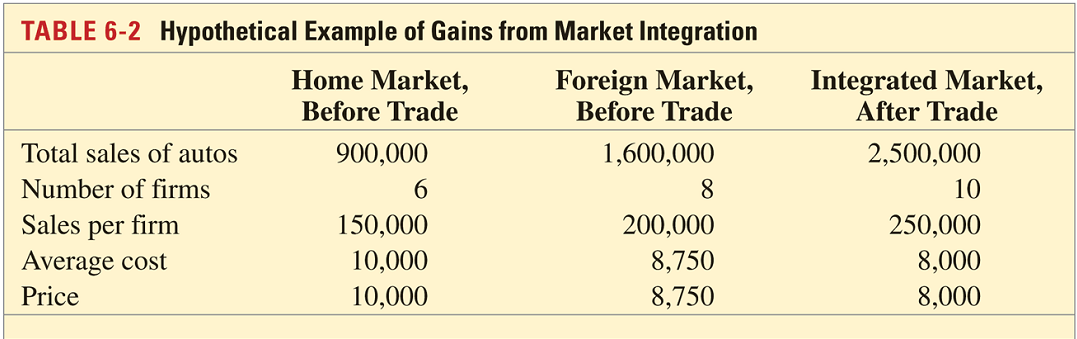
\includegraphics[width=10cm]{fig/krugman/lec6-17}
\end{figure}

\end{itemize}
\end{frame}

\begin{frame}{Implications for the Structure of Trade }


In neoclassical trade models (Ricardian, Heckscher-Ohlin) countries
specialize in certain industries and hence trade is inter-industry
trade 

Example: Cloth is capital- intensive relative to Food 
\begin{figure}
\centering{}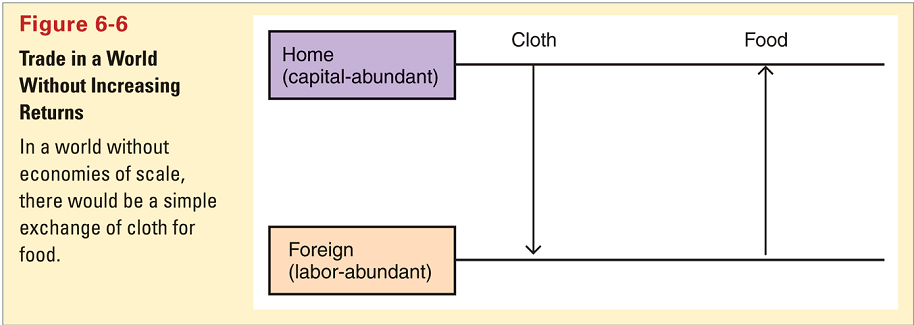
\includegraphics[width=12cm]{fig/krugman/lec6-18}
\end{figure}



\end{frame}

\begin{frame}{Intra -Industry Trade }

\begin{itemize}
\item Now suppose that \textbf{\textcolor{red}{cloth is not a homogenous
good}}, and the global cloth industry is better described by the monopolistic
competition model 
\item In equilibrium, Home and Foreign will produce different varieties
of clothes (as in our example)
\item So Home will not only export cloth, it will now import it as well!
\item Hence, \textbf{\textcolor{red}{with IRS}} and imperfect competition,
trade also occurs within the cloth industry: \textbf{\textcolor{red}{intra-industry
trade}}
\end{itemize}
\end{frame}

\begin{frame}{Inter and Intra -Industry Trade}

\begin{itemize}
\item Still, Home is capital- abundant, and hence we expect it to be a net
exporter of cloth and net importer of food (as in H - O model) 
\begin{figure}
\centering{}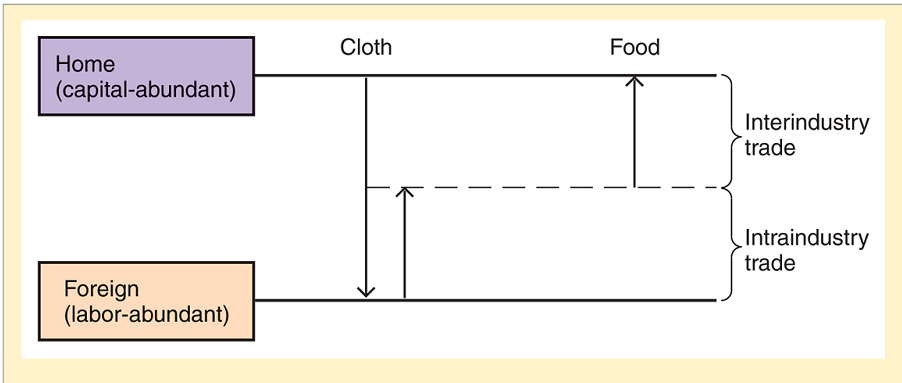
\includegraphics[width=11cm]{fig/krugman/lec6-19}
\end{figure}

\end{itemize}
\end{frame}

\begin{frame}{Recap on Pattern of Trade }

\begin{itemize}
\item Gains from inter-industry trade reflect traditional comparative advantage. 
\item Gains from intra-industry trade reflect economies of scale and wider
consumer choices. 
\item What determines the relative size of inter-industry vs. intra-industry
trade? 

\begin{itemize}
\item Countries with similar relative amounts of factors of production are
predicted to have little inter-industry trade, so most trade is intra-industry
trade 
\item Less trivially, larger and more similar countries will also feature
a larger volume of intra- industry trade 

\begin{itemize}
\item gains from economies of scale are larger 
\end{itemize}
\end{itemize}
\end{itemize}
\end{frame}

\begin{frame}{Evidence: Intra-Industry Trade}

\begin{itemize}
\item Some industries have more intra-industry trade than others: 

\begin{itemize}
\item Larger in skill-, technology-, and capital-intensive industries 
\item These tend to be the industries where economies of scale, imperfect
competition and product differentiation are more relevant 
\end{itemize}
\item Also, share of intra-industry trade with U.S. is larger for countries
with similar relative amounts of skilled labor, technology and physical
capital 
\item Problem: “pseudo- intraindustry trade” (vertical fragmentation) 
\end{itemize}
\end{frame}

\begin{frame}{Some Examples }


\begin{figure}
\centering{}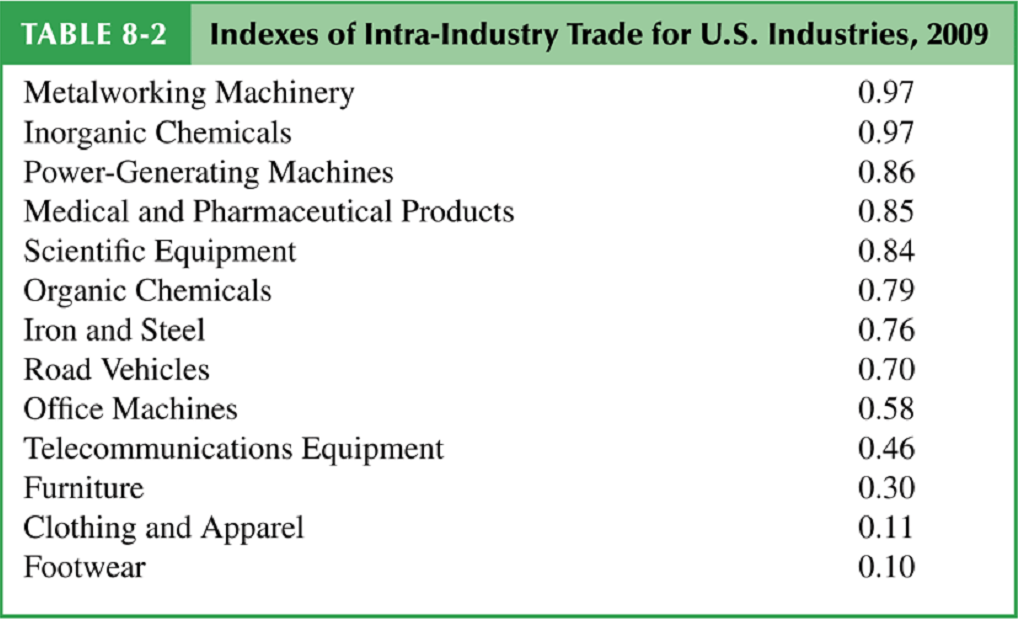
\includegraphics[width=10cm]{fig/krugman/lec6-20}
\end{figure}

\end{frame}

\begin{frame}{Implications for Income Distribution }

\begin{itemize}
\item Remember that in the H-O model, inter-industry trade generated winners
and losers 
\item In the model above, all consumers benefit from trade (perhaps some
more than others depending on their “love-for-variety”) 
\item So whenever the share of intra- industry trade is large, we may expect
welfare gains to be more evenly distributed
\item Two caveats: 

\begin{itemize}
\item Some models with IRS and imperfect competition generate wasteful two-way
trade flows (see Brander and Krugman, 1983) 
\item Trade integration may reduce the number of “local varieties” 
\end{itemize}
\end{itemize}
\end{frame}





\end{document}
